\documentclass[10.5pt]{article}
\usepackage{amsmath,amssymb}
\usepackage{fontspec}
\usepackage{xcolor}
\usepackage{graphicx}
\usepackage{tabularx}
\usepackage{enumitem}
\usepackage{multicol}
\usepackage{fancyhdr}
\usepackage[many]{tcolorbox}
\usepackage[a4paper, top=16mm, bottom=20mm, left=13mm, right=13mm]{geometry}
\setlength{\parindent}{0pt}
\setlength{\parskip}{0pt}
\IfFontExistsTF{Noto Sans KR}{\setmainfont{Noto Sans KR}}{\setmainfont{Malgun Gothic}}
\definecolor{examBlue}{HTML}{245BD1}
\definecolor{ruleGray}{gray}{0.6}
\pagestyle{fancy}
\fancyhf{}
\setlength{\headheight}{22pt}
\setlength{\headsep}{8pt}
\setlength{\footskip}{28pt}
\makeatletter
\renewcommand{\headrule}{\hbox to\headwidth{\color{examBlue}\leaders\hrule height \headrulewidth\hfill}}
\renewcommand{\footrule}{\hbox to\headwidth{\color{ruleGray}\leaders\hrule height \footrulewidth\hfill}}
\makeatother
\renewcommand{\headrulewidth}{0.8pt}
\renewcommand{\footrulewidth}{0.4pt}
\fancyhead[L]{고1}\fancyhead[C]{모의고사}\fancyhead[R]{시험지}\fancyfoot[L]{수학학습실}\fancyfoot[C]{\thepage}\fancyfoot[R]{https://www.math114.net}

\setlength{\columnsep}{9mm}
\setlength{\columnseprule}{0.5pt}
\setlist[enumerate,1]{label=\textcolor{examBlue}{\Large\bfseries\arabic*.}, leftmargin=*, itemsep=0.2em, topsep=0em, parsep=0pt}
\begin{document}

\thispagestyle{fancy}
\vspace*{-6mm}
\noindent{\bfseries\Large 수학학원명}\hfill{\bfseries 모의고사}
\begin{center}{\bfseries\LARGE 시험지}\end{center}
{\color{examBlue}\rule{\linewidth}{0.9pt}}
\vspace{2mm}
\renewcommand{\arraystretch}{1.35}
\begin{tabularx}{\linewidth}{@{}lX lX lX lX@{}}
이름 & \hrulefill & 날짜 & \hrulefill & 시간 & \hrulefill & 단원 & \hrulefill \\
\end{tabularx}
\vspace{8mm}
\begin{multicols}{2}
\begin{enumerate}
\item \leavevmode\begin{minipage}[t]{\linewidth}
$5^{\sqrt{2}+1} \times\left(\frac{1}{5}\right)^{\sqrt{2}}$ 의 값은? [2점]
\vspace{0.5em}
\begin{enumerate}[label={\textcircled{\arabic*}}, itemsep=0.2em, topsep=0.2em, leftmargin=*, align=left]
\item $\frac{1}{25}$
\item $\frac{1}{5}$
\item 1
\item 5
\item 25
\end{enumerate}
\par\vspace{12\baselineskip}
\end{minipage}
\item \leavevmode\begin{minipage}[t]{\linewidth}
함수 $f(x)=x^{2}-4 x+2$ 에 대하여 $\lim _{h \rightarrow 0} \frac{f(4+h)-f(4)}{h}$ 의 값은? [2점]
\vspace{0.5em}
\begin{enumerate}[label={\textcircled{\arabic*}}, itemsep=0.2em, topsep=0.2em, leftmargin=*, align=left]
\item 1
\item 2
\item 3
\item 4
\item 5
\end{enumerate}
\par\vspace{12\baselineskip}
\end{minipage}
\item \leavevmode\begin{minipage}[t]{\linewidth}
수열 $\left\{a_{n}\right\}$ 에 대하여 $\sum_{k=1}^{6}\left(2 a_{k}-1\right)=30$ 일 때, $\sum_{k=1}^{6} a_{k}$ 의 값은?
\vspace{0.5em}
\begin{enumerate}[label={\textcircled{\arabic*}}, itemsep=0.2em, topsep=0.2em, leftmargin=*, align=left]
\item 2
\item 6
\item 10
\item 14
\item 18
\end{enumerate}
\par\vspace{12\baselineskip}
\end{minipage}
\item \leavevmode\begin{minipage}[t]{\linewidth}
닫힌구간 $[-2,2]$ 에서 정의된 함수 $y=f(x)$ 의 그래프가 그림과 같다. $\lim _{x \rightarrow 0-} f(x)+\lim _{x \rightarrow 1+} f(x)$ 의 값은? [3점]
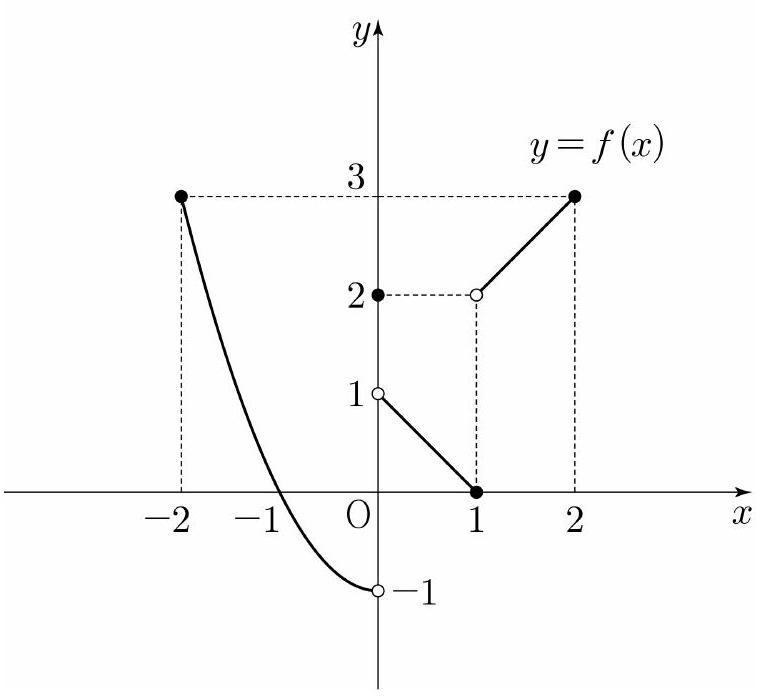
\includegraphics[width=0.8\linewidth]{images/img_cf54ac5ce2d59f5127376da2222d433b.jpg}
\vspace{0.5em}
\begin{enumerate}[label={\textcircled{\arabic*}}, itemsep=0.2em, topsep=0.2em, leftmargin=*, align=left]
\item 1
\item 2
\item 3
\item 4
\item 5
\end{enumerate}
\par\vspace{12\baselineskip}
\end{minipage}
\item \leavevmode\begin{minipage}[t]{\linewidth}
함수 $f(x)=\left(x^{2}+2\right)\left(x^{2}+x-3\right)$ 에 대하여 $f^{\prime}(1)$ 의 값은? [3점]
\vspace{0.5em}
\begin{enumerate}[label={\textcircled{\arabic*}}, itemsep=0.2em, topsep=0.2em, leftmargin=*, align=left]
\item 6
\item 7
\item 8
\item 9
\item 10
\end{enumerate}
\par\vspace{12\baselineskip}
\end{minipage}
\item \leavevmode\begin{minipage}[t]{\linewidth}
곡선 $y=x^{3}-5 x^{2}+6 x$ 위의 점 $(3,0)$ 에서의 접선이 점 $(5, a)$ 를 지날 때, $a$ 의 값은? [3점]
\vspace{0.5em}
\begin{enumerate}[label={\textcircled{\arabic*}}, itemsep=0.2em, topsep=0.2em, leftmargin=*, align=left]
\item 6
\item 7
\item 8
\item 9
\item 10
\end{enumerate}
\par\vspace{12\baselineskip}
\end{minipage}
\item \leavevmode\begin{minipage}[t]{\linewidth}
다항함수 $f(x)$ 의 한 부정적분을 $F(x)$ 라 하고, 함수 $2 f(x)+1$ 의 한 부정적분을 $G(x)$ 라 하자. $G(3)=2 F(3)$ 일 때, $G(5)-2 F(5)$ 의 값은?
\vspace{0.5em}
\begin{enumerate}[label={\textcircled{\arabic*}}, itemsep=0.2em, topsep=0.2em, leftmargin=*, align=left]
\item 1
\item 2
\item 3
\item 4
\item 5
\end{enumerate}
\par\vspace{12\baselineskip}
\end{minipage}
\item \leavevmode\begin{minipage}[t]{\linewidth}
$\cos (\theta-\pi)=\frac{3}{5}$ 이고 $\tan \theta<0$ 일 때, $\sin \theta$ 의 값은?
\vspace{0.5em}
\begin{enumerate}[label={\textcircled{\arabic*}}, itemsep=0.2em, topsep=0.2em, leftmargin=*, align=left]
\item $-\frac{4}{5}$
\item $-\frac{3}{5}$
\item $\frac{1}{5}$
\item $\frac{3}{5}$
\item $\frac{4}{5}$
\end{enumerate}
\par\vspace{12\baselineskip}
\end{minipage}
\item \leavevmode\begin{minipage}[t]{\linewidth}
두 양수 $a, b$ 가 $\log _{\sqrt{2}} a+\log _{2} b=2, \quad \log _{2} a+\log _{2} b^{2}=7$ 을 만족시킬 때, $a \times b$ 의 값은?
\vspace{0.5em}
\begin{enumerate}[label={\textcircled{\arabic*}}, itemsep=0.2em, topsep=0.2em, leftmargin=*, align=left]
\item 2
\item 4
\item 8
\item 16
\item 32
\end{enumerate}
\par\vspace{12\baselineskip}
\end{minipage}
\item \leavevmode\begin{minipage}[t]{\linewidth}
시각 $t=0$ 일 때 원점에서 출발하여 수직선 위를 움직이는 점 P 가 있다. 시각이 $t(t \geq 0)$ 일 때 점 P 의 속도 $v(t)$ 가
\[v(t)=3 t^{2}-10 t+7\]
이다. <보기>에서 옳은 것만을 있는 대로 고른 것은? [4점]
\begin{tcolorbox}[colback=white, colframe=black, boxrule=0.5pt, arc=2pt, boxsep=3pt, left=4pt, right=4pt, top=3pt, bottom=3pt]
ㄱ. 시각 $t=1$ 일 때 점 P 의 운동 방향이 바뀐다.\\
ㄴ. 시각 $t=1$ 일 때 점 P 의 위치는 3 이다.\\
ㄷ. 시각 $t=0$ 에서 $t=2$ 까지 점 P 가 움직인 거리는 4 이다.
\end{tcolorbox}
\vspace{0.5em}
\begin{enumerate}[label={\textcircled{\arabic*}}, itemsep=0.2em, topsep=0.2em, leftmargin=*, align=left]
\item ᄀ
\item ᄀ, ᄂ
\item ᄀ, ᄃ
\item ᄂ, ᄃ
\item ᄀ, ᄂ, ᄃ
\end{enumerate}
\par\vspace{12\baselineskip}
\end{minipage}
\item \leavevmode\begin{minipage}[t]{\linewidth}
모든 항이 양수인 등비수열 $\left\{a_{n}\right\}$ 의 첫째항부터 제 $n$ 항까지의 합을 $S_{n}$ 이라 하자.
\[
a_{2}=1, \quad \sum_{k=1}^{6}(-1)^{k} S_{k}=21
\]
일 때, $S_{2}+S_{7}$ 의 값은? [4점]
\vspace{0.5em}
\begin{enumerate}[label={\textcircled{\arabic*}}, itemsep=0.2em, topsep=0.2em, leftmargin=*, align=left]
\item 61
\item 63
\item 65
\item 67
\item 69
\end{enumerate}
\par\vspace{12\baselineskip}
\end{minipage}
\end{enumerate}\end{multicols}\end{document}